\documentclass[a4paper,11pt,hidelinks]{article}
\usepackage[utf8]{inputenc}  % Linux, macOS: enable non-English characters
%\usepackage[latin1]{inputenc}    % Windows: enable non-English characters
\usepackage[left=2.5cm,right=2.5cm,top=2.5cm,bottom=2.5cm]{geometry}
\usepackage[british]{babel}

%% Instructions are preceded by "%%", whether you use LaTeX or not!

%\renewcommand{\thepart}{\arabic{part}}
\renewcommand{\thesection}{\Alph{section}}

%% Useful packages:
\usepackage[boxed]{algorithm}   % drop [boxed] is no box around algorithm wanted
\usepackage[noend]{algorithmic} % drop [noend] if endif, endwhile, etc wanted
\renewcommand{\algorithmiccomment}[1]{\hfill // #1}
\usepackage{alltt}
\usepackage{amsmath}
\usepackage{amssymb}
\usepackage{array}
\usepackage[british]{babel}
\usepackage{booktabs}
\usepackage{cancel}  % provides \cancel
\usepackage{xcolor}  % supersedes color
\usepackage{colortbl}  % provides \cellcolor
\usepackage[nocenter]{cwpuzzle}  % provides Sudoku
\usepackage{graphicx}  % provides \includegraphics
\usepackage{logicpuzzle}  % provides kakuro
\definecolor{kakuro}{RGB}{155,206,167}
\kakurosetup{color=kakuro}
\usepackage{mathtools} \mathtoolsset{showonlyrefs}  % provides \coloneqq
\usepackage{multicol}
\usepackage{multirow}
\usepackage{pdflscape}  % provides "landscape" environment
\usepackage{pgfplots} \pgfplotsset{compat=1.12}  % was 1.9, but gave errors?!
\usepackage{rotating}  % provides "sideways[table]" environments
\usepackage{tikz}
\usetikzlibrary{arrows,automata,calc,trees,positioning,decorations.markings}
\usepackage{xspace}
\usepackage{xstring}
\usepackage{hyperref}
\hypersetup{linkcolor=black}  % should always be last package

%% Fancy characters:
\usepackage{pifont}
%\newcommand{\scissors}{\ding{36}}
%\newcommand{\phone}{\ding{37}}
%\newcommand{\aircraft}{\ding{40}}
%\newcommand{\envelope}{\ding{41}}
\newcommand{\handpoint}{\ding{43}}
%\newcommand{\victory}{\ding{44}}
%\newcommand{\handwrite}{\ding{45}}
\newcommand{\tick}{\ding{51}}
\newcommand{\notick}{\ding{55}}
\DeclareSymbolFont{extraup}{U}{zavm}{m}{n}
%\DeclareMathSymbol{\varclubsuit}{\mathalpha}{extraup}{84}
%\DeclareMathSymbol{\varspadesuit}{\mathalpha}{extraup}{85}
\DeclareMathSymbol{\varheartsuit}{\mathalpha}{extraup}{86}
\DeclareMathSymbol{\vardiamondsuit}{\mathalpha}{extraup}{87}

%% Styles:
\newcommand{\important}[1]{\textcolor{red}{#1}}
\newcommand{\stressed}[1]{\textbf{\textit{#1}}}
\newcommand{\todo}[1]{\textcolor{green}{#1}}  % show to-do items in green
%\newcommand{\todo}[1]{}                      % omit to-do items
\newcommand{\done}[1]{\textcolor{blue}{#1}}   % show done  items in blue
%\newcommand{\done}[1]{#1}                    % show done  items in black

%% Tools and Languages:
\newcommand{\FlatZinc}{Flat\-Zinc\xspace}
\newcommand{\Gecode}{Gecode\xspace}
%\newcommand{\GIST}{GIST\xspace}
\newcommand{\MiniCP}{Mini\-CP\xspace}
\newcommand{\MiniModel}{Mini\-Model\xspace}
\newcommand{\MiniZinc}{Mini\-Zinc\xspace}
\newcommand{\Python}{Python\xspace}

%% Algorithms:
\newcommand{\EndIf}{\textbf{~endif}}
\newcommand{\Function}{\textbf{function~}}
\newcommand{\IfThen}[2]{\If#1\Then#2\EndIf}  % use when \IF unsuitable
\newcommand{\In}{\textbf{~in~}}
\newcommand{\Invariant}[1]{{\bf invariant:} #1}
%\newcommand{\IsAssigned}{\gets}
\newcommand{\IsAssigned}{\coloneqq}
\newcommand{\Let}[2]{\textbf{let~}#1\In#2}
\newcommand{\PostCond}[1]{\textbf{post:} #1}
\newcommand{\PreCond}[1]{\textbf{pre:} #1}
\newcommand{\Return}{\textbf{return~}}  % use when \RETURN unsuitable
\newcommand{\Select}{\textbf{select}}
\newcommand{\Variant}[1]{{\bf variant:} #1}

%% Automata:
\newcommand{\Alphabet}{\Sigma}
\newcommand{\Alternation}[2]{#1|#2}           % of regular expressions
\newcommand{\Concat}[2]{#1 \cdot #2}          % of strings
\newcommand{\DFA}{\mathcal{A}}
\newcommand{\EmptyString}{\epsilon}
\newcommand{\Kleene}[1]{#1^*}                 % of a regular expression
\newcommand{\Language}[1]{\mathcal{L}({#1})}  % of a regular expression
\newcommand{\RegEx}[1]{\mathbf{#1}}           % transforms symbol into reg.ex.

%% CP & Gecode & MiniCP & MiniZinc:
\newcommand{\AllDifferent}{\Constraint{AllDifferent}}  % MiniCP
\newcommand{\AnyCond}[1]{\text{Any}(#1)}  % Gecode
\newcommand{\BinPacking}{\Constraint{binpacking}}  % Gecode
\newcommand{\BoundedCond}[1]{\text{Bounded}(#1)}  % Gecode
\newcommand{\Channel}{\Constraint{channel}}  % Gecode
%\newcommand{\Circuit}{\Constraint{circuit}}  % Gecode
\newcommand{\Circuit}{\Constraint{Circuit}}  % MiniCP
\newcommand{\CondSet}[1]{\text{PropConds}(#1)}  % Gecode
\newcommand{\Conds}[2]{\text{Conds}(#1,#2)}  % Gecode
%\newcommand{\Constraint}[1]{\textsc{#1}}
\newcommand{\Constraint}[1]{\texttt{#1}}
%\newcommand{\Cumulative}{\Constraint{cumulative}}  % Gecode
\newcommand{\Cumulative}{\Constraint{Cumulative}}  % MiniCP
\newcommand{\DepProps}{\textit{DepProps}}  % Gecode
\newcommand{\DFE}{\text{DFE}}  % Gecode
\newcommand{\Disjunctive}{\Constraint{Disjunctive}}  % MiniCP
\newcommand{\Distinct}{\Constraint{distinct}}  % Gecode
\newcommand{\Domain}[1]{\textnormal{dom}(#1)}
%\newcommand{\Element}{\Constraint{element}}  % Gecode
\newcommand{\Element}{\Constraint{Element}}  % MiniCP
\newcommand{\Extensional}{\Constraint{extensional}}  % Gecode
\newcommand{\Failed}{\text{Failed}}  % Gecode
\newcommand{\FailedCond}[1]{\text{Failed}(#1)}  % Gecode
\newcommand{\FixedCond}[1]{\text{Fixed}(#1)}  % Gecode
\newcommand{\Fixpoint}{\text{AtFixpt}}  % Gecode
\newcommand{\GlobalCardinality}{\Constraint{count}}  % Gecode
\newcommand{\Linear}{\Constraint{linear}}  % Gecode
\newcommand{\MaxCond}[1]{\text{Max}(#1)}  % Gecode
\newcommand{\MinCond}[1]{\text{Min}(#1)}  % Gecode
\newcommand{\ModVars}{\textit{ModVars}}  % Gecode
\newcommand{\NoneCond}[1]{\text{None}(#1)}  % Gecode
\newcommand{\NValues}{\Constraint{nvalues}}  % Gecode
\newcommand{\Path}{\Constraint{path}}  % Gecode
\newcommand{\Precede}{\Constraint{precede}}  % Gecode
\newcommand{\Propagate}{\text{Propagate}}
%\newcommand{\Reifies}[2]{#1\Leftrightarrow#2}
\newcommand{\Reifies}[2]{#2\Leftrightarrow#1}  % layout as in MiniZinc
\newcommand{\Stores}{\mathbb{S}}
\newcommand{\Subsumed}{\text{Subsumed}}  % Gecode
\newcommand{\Sum}{\Constraint{Sum}}  % MiniCP
\newcommand{\Table}{\Constraint{Table}}  % MiniCP
\newcommand{\Unary}{\Constraint{unary}}  % Gecode
\newcommand{\Unknown}{\text{Unknown}}  % Gecode
\newcommand{\Variables}[1]{\text{var}(#1)}

%% Mathematics:
\newcommand{\AbsValue}[1]{\left\lvert#1\right\rvert}
\newcommand{\Cardinality}[1]{\left\lvert#1\right\rvert}
%\newcommand{\Cardinality}[1]{\##1}
\newcommand{\Ceiling}[1]{\left\lceil#1\right\rceil}
\newcommand{\Else}{\textbf{~else~}}
\newcommand{\EmptySet}{\varnothing}
\newcommand{\Floor}[1]{\left\lfloor#1\right\rfloor}
\newcommand{\GeqLex}{\geq_{\Lex}}
\newcommand{\If}{\textbf{if~}}
\newcommand{\Iff}{\Leftrightarrow}
\newcommand{\IfThenElse}[3]{\If#1\Then#2\Else#3}
\newcommand{\Implies}{\Rightarrow}
\newcommand{\Int}{\mathbb{Z}}
\newcommand{\Inter}{\cap}
\newcommand{\Iverson}[1]{\red{\left[\textcolor{black}{#1}\right]}}
\newcommand{\LeqLex}{\leq_{\Lex}}
\newcommand{\Lex}{\textnormal{lex}}
\newcommand{\LtLex}{<_{\Lex}}
\newcommand{\Nat}{\mathbb{N}}
\newcommand{\Oh}[1]{\mathcal{O}(#1)}
\newcommand{\Sequence}[1]{\left[#1\right]}
\newcommand{\Set}[1]{\left\{#1\right\}}
\newcommand{\SetComp}[2]{\Set{#1\SuchThat#2}}
\newcommand{\SuchThat}{\mid}
\newcommand{\Then}{\textbf{~then~}}
\newcommand{\Tuple}[1]{\left\langle#1\right\rangle}
\newcommand{\Union}{\cup}
\newcommand{\Where}{\textbf{~~where~~}}

\usepackage{listings}
\usepackage{courier} % \texttt{...} gives thinner text and /\ displays OK

\newcommand\mznfont{\fontfamily{pcr}\selectfont}

\lstdefinelanguage{Mzn}
{
  morekeywords={
  %
  array, par, var, opt, constraint, solve, satisfy, minimize,
  maximize, output, include, let, in, set, of, if, then, else, elseif, endif,
  ann, annotation, bool, enum, float, int, string, where, function,
  predicate, true, false, not, assert, trace,
  % ???:
  any, list, op, record, test, tuple, type,
  %
  },
  %
  keywords=[2]{
  %
  forall, exists, xor, xorall, iffall, clause,
  all_different, all_different_int,
  all_different_except_0, all_different_except, all_equal,
  nvalue, diffn,
  at_least, at_most, exactly, % deprecated!
  count, count_eq, count_leq, count_geq, count_gt, among,
  global_cardinality, global_cardinality_closed,
  global_cardinality_low_up, global_cardinality_low_up_closed,
  element, regular, regular_nfa, table, inverse, inverse_in_range,
  bin_packing, bin_packing_capa, bin_packing_load, knapsack,
  cumulative, disjunctive, circuit, subcircuit, dpath,
  decreasing, increasing,
  strictly_decreasing, strictly_increasing,
  lex_less, lex_lesseq, lex_greater, lex_greatereq, lex2, strict_lex2,
  value_precede, value_precede_chain,
  symmetry_breaking_constraint, implied_constraint, redundant_constraint,
  sort, arg_sort, among, sliding_sum,
  int_ne, int_lt_reif, int_lin_eq, int_lin_eq_reif, bool_lin_eq, int_eq_imp,
  bool_imply, array_bool_or,
  in_set, subset, superset, partition_set, member,
  % from ???:
  abort,
  acosh, asin, atan, cos, cosh, sin, sinh, tan, tanh,
  array_intersect, array_union,
  array1d, array2d, array3d, array4d, array5d, array6d,
  bool2int, int2float, set2array,
  abs, div, mod, pow, exp, sqrt, ln, log, log2, log10,
  ceil, floor, round,
  enum_next,
  min, max, length, product, sum,
  dom, dom_array, dom_size, fix, is_fixed,
  index_set, index_set_1of2, index_set_2of2,
  index_set_1of3, index_set_2of3, index_set_3of3, index_set_6of6,
  concat, reverse, join,
  lb, lb_array, ub, ub_array,
  show, show2d, show_int, show_float,
  card, intersect, union, diff, symdiff,
  % annotations:
  add_to_output,
  is_defined_var, output_var, var_is_introduced, defines_var, promise_total,
  value_propagation, bounds_propagation, domain_propagation,
  bool_search, int_search, seq_search,
  set_search, input_order, first_fail, anti_first_fail, smallest,
  largest, occurrence, most_constrained, max_regret, indomain_min,
  indomain_max, indomain_middle, indomain_median, indomain,
  indomain_random, indomain_split, indomain_reverse_split,
  indomain_interval, outdomain_max, outdomain_median, outdomain_min,
  outdomain_random, complete, restart_constant, relax_and_reconstruct
  % 
  },
  sensitive=true,
  basicstyle=\mznfont,
  commentstyle=\color[rgb]{0.9,0.1,0.1},
  keywordstyle=\color[rgb]{0,0.5,0},
  keywordstyle=[2]\color{blue},
  stringstyle=\color{orange},
  tabsize=2,
  frame=none,
  % identifierstyle = \it,
  numbers=left,
  stepnumber=1,
  numberstyle=\tiny,
  numbersep=5pt,
  xleftmargin=0pt, % numbers will be in the margins!
  columns=fixed, % same width for all characters
  % columns=flexible,
  % columns=fullflexible,
  morecomment=[l]{\%},
  morestring=[b]",
  % morestring=[d]',
  showstringspaces=false,
  mathescape=true,
  breaklines=true,
  % prebreak=\raisebox{0ex}[0ex][0ex]{\ensuremath{\space\red{\swarrow}}},%\hookrightarrow
  %postbreak=\raisebox{0ex}[0ex][0ex]{\ensuremath{\hookrightarrow\space}},%\hookrightarrow
  breakatwhitespace=true,
  breakindent=10pt, % was: 20pt
  moredelim=**[is][\color{Melon}]{@}{@},
  escapeinside={{<@}{@>}}
}
%% Write "\begin{frame}[fragile]" for a slide using either of the
%% following two listing environments, which have unnumbered
%% respectively numbered lines:
\lstnewenvironment{mzn}[1][]{\lstset{language=Mzn,#1}}{}
\lstnewenvironment{mznno}[1][]{\lstset{language=Mzn,numbers=none,xleftmargin=0pt,#1}}{}
%% Inline a code snippet, without respectively with the comprehension bar (|):
\newcommand{\mzninline}[1]{\lstinline[{language=Mzn}]|#1|}
\newcommand{\mzninlinebar}[1]{\lstinline[{language=Mzn}]!#1!}


\renewcommand{\todo}[1]{\textcolor{blue}{#1}} %% Use for spotting placeholders
%\renewcommand{\todo}[1]{#1}                  %% Use for the submitted report

\newcommand{\Problem}{\todo{Problem}\xspace}  %% Plug in your project name

\title{\textbf{Modelling for Combinatorial Optimisation (1DL451) \\
    Uppsala University -- Autumn~2025 \\
    Report for the Project
    by Team~\todo{t}: \\                      %% Replace t by your team number
    \Problem
  }
}

%% Replace by your name(s) and choose the encoding of line 2 or line 3:
\author{\todo{Clara CLÄVER and Whiz KIDD}}

\date{\today}

\begin{document}

\maketitle

% -------------------------------------------------------------------------

\section{\Problem}

%% Describe your project problem, in your own words, citing the source
%% of the problem and of every included third-party picture.

\todo{\dots\ Reply \dots}

% -------------------------------------------------------------------------

\section{Approach}

%% Describe your approach to your project problem.
%% If your approach is just a single model (like for the assignments),
%% then just say so and follow the model instructions of demoReport.pdf,
%% else describe your software pipeline -- with pre-processing,
%% solving (possibly on a sequence of models), and post-processing --
%% and follow the model instructions of demoReport.pdf for _each_ model.
%% Either way, upload _all_ code and data to Studium (_except_ for the
%% initial report), but _only_ import your model(s) into the report itself).
%% The report must be about exactly one approach (and this word is _not_
%% a synonym for 'viewpoint') and must _not_ describe all false starts.

\todo{\dots\ Reply \dots}

%% Find in demoReport.pdf the instructions on prescribed comments within a model.
Our model is given in Listing~\ref{model:project}: it has the
prescribed comments as per the scope (Topics~1 to~8) of the project,
it has the name \todo{\texttt{project.mzn}}             %% Replace the filename
and the imposed structure of the provided skeleton model
\texttt{project-skeleton.mzn}%
%% Comment away the following line for the initial report
, and it is uploaded to Studium.

%% Set the numeric parameters so that the copyright notice is skipped:
\lstinputlisting[language=Mzn, firstline=5, firstnumber=5,
caption={A \MiniZinc model for \todo{\dots} },
label=model:project]{project-skeleton.mzn} %% Replace the filename

\paragraph{Symmetries.}
%% * Identify the problem symmetries, which exist for every viewpoint.
%% * Identify the model symmetries, which are introduced by your viewpoint.
%% * For each identified symmetry, state:
%%   + whether it is a value symmetry or a variable symmetry
%%     (an example of which is an index symmetry, say a row or column symmetry);
%%   + whether it is a full or partial symmetry.
\todo{\dots\ problem symmetry \dots\ model symmetry \dots\ value /
  variable / index / row / column symmetry \dots\ full / partial
  symmetry \dots}

\paragraph{Efficiency.}
%% * State the impact, or justify the absence, of
%%   + implied constraints, and
%%   + symmetry-breaking constraints.
%%   Do _not_ test them on CBLS backends, such as Yuck, which ignore them.
%% * State the impact, or justify the absence, of
%%   + reasoning annotations, and
%%   + search annotations.
%%   Restrict your tests to the CP backend Gecode.
\todo{\dots\ implied constraints \dots\ symmetry-breaking constraints
  \dots\ reasoning annotations \dots\ search annotations \dots}

\paragraph{Checklist.}
%% For each model feature covered by advice in the checklists of Topics 2 & 3:
%% how do you argue that it does not matter?
\todo{\dots\ Reply (and we understand that we may lose points if there
  are such model features that we did not detect and discuss) \dots}

\paragraph{Correctness.}
%% How do you argue that your approach is correct?
%% For example, do you use a checker based on another model, such as a
%% model by another team or a linearisation of a MIP model found somewhere?
%% Do you use the same new instances as another team?
%% If it is a satisfaction problem: do you compare the numbers of
%% solutions with numbers found somewhere or reported by another team?
%% If it is an optimisation problem: do you compare objective values that
%% are proven optimal before timing out (respectively objective values
%% known when timing out) with optimal objective values (respectively
%% best-known objective values) found somewhere or reported by another
%% team?)
\todo{\dots\ Reply \dots}

% -------------------------------------------------------------------------

\section{Evaluation}

%% Hint: Under Linux, do lscpu to find CPU information.  Under macOS,
%% you find CPU information via "About This Mac" in the Apple menu.
%% 
%% If different hardware was used for different experiments, then justify
%% this and replicate a paragraph like this one within each relevant section.

All experiments were run under Linux Ubuntu~22.04.5 ($64$~bit) on an
Intel Xeon E5520 of $2.27$~GHz, with $4$~processors of $4$~cores each,
with a $70$~GiB RAM and an $8$~MiB L3 cache (a ThinLinc computer of the
IT department). % barany.it.uu.se

\newcommand{\TimeOut}{\todo{6,000,000}} % in CPU milliseconds  %% Choose a value

%% You _must_ use the script of our cheatsheet: it conducts the
%% experiments and generates a result table (see the LaTeX source code
%% of the table below}) that is automatically imported (rather than
%% manually copied) into your report, so each time you change the
%% model, it suffices to re-run that script and re-compile your
%% report, without any tedious number copying!

Table~\ref{tab:res} gives our results.
The time-out was~\TimeOut~milliseconds.

%\begin{landscape}  %% Uncomment this if the table is too wide!
\begin{table}[t]
  \centering
  \resizebox{\columnwidth}{!}{\fontfamily{pcr}\selectfont\small
    \begin{tabular}{rrrrrrrrrrrrr}
      Backend
	& \multicolumn{2}{c}{Chuffed}
	& \multicolumn{2}{c}{CP-SAT}
	& \multicolumn{2}{c}{Gecode}
	& \multicolumn{2}{c}{Gurobi}
	& \multicolumn{2}{c}{PicatSAT}
	& \multicolumn{2}{c}{Yuck}
\\
	\cmidrule(lr){2-3}
	\cmidrule(lr){4-5}
	\cmidrule(lr){6-7}
	\cmidrule(lr){8-9}
	\cmidrule(lr){10-11}
	\cmidrule(lr){12-13}
        \dots
	& \texttt{obj} & time
	& \texttt{obj} & time
	& \texttt{obj} & time
	& \texttt{obj} & time
	& \texttt{obj} & time
	& \texttt{obj} & time
\\
        \midrule
        \dots
	& \dots	& \dots
	& \dots	& \dots
	& \dots	& \dots
	& \dots	& \dots
	& \dots	& \dots
	& \dots	& \dots
\\
  %% Replace the filename
    \end{tabular}}
  \caption{Results for our approach to \Problem,
    which is a \todo{minimisation / maximisation / satisfaction} problem.
    % 
    In each \texttt{time} column: if the reported time is less than
    the time-out (\TimeOut~milliseconds here), then the
    %% For a CSP, tweak the following snippet as in Table 1 for Assignment 1:
    \todo{objective value in the corresponding \texttt{obj} column was
      \emph{proven} optimal};
    % 
    else the timing out is indicated by \texttt{t/o} and the
    %% For a CSP, tweak the following snippet as in Table 1 for Assignment 1:
    \todo{objective value is either the best one found but \emph{not}
      proven optimal before timing out,
      or~`\texttt{-}' indicating that no feasible solution was found
      before timing out}.
    % 
    Boldface indicates the
    %% For a CSP, replace by "fastest time":
    \todo{best performance (time or objective value)}
    %
    on each row.
    % 
  }
  \label{tab:res}
\end{table}
%\end{landscape}

\paragraph{Which backends win overall, and how do you draw that conclusion?}
\todo{\dots\ Reply \dots}

\paragraph{How do the backends scale, and how do you draw that conclusion?}
\todo{\dots\ Reply \dots}

\paragraph{Does the difficulty of instances monotonically increase
  with their size, and how do you draw that conclusion?}
\todo{\dots\ Reply \dots}

\paragraph{How suitable is local search compared to systematic search,
  and how do you draw that conclusion?}
\todo{\dots\ Reply \dots}

\paragraph{Are there any contradictions between the results?}
\todo{\dots\ Reply \dots}

\paragraph{Are there any occurrences of `ERR' within the results generated
  by the experiment script?}
%% If so, then first try and troubleshoot on your own by running the
%% incriminated backend manually (within the IDE or at the command
%% line by using the --solver flag of the minizinc command) and
%% interpreting the error message.  If you cannot resolve the error,
%% then you _must_ state here for each occurrence of ERR when and how
%% you received a teacher's _prior_ approval to include it, and you
%% ought to make an error report in the final section.
\todo{\dots\ Reply \dots}

% -------------------------------------------------------------------------

%% Optional:

\bigskip
\section*{Feedback to the Teachers}

%% Please write a paragraph, which will _not_ be graded, describing your
%% experience with this report: which aspects were too difficult or
%% too easy, and which aspects were interesting or boring?  This will
%% help us improve the course for the next year.

\todo{\dots\ Reply \dots}

% -------------------------------------------------------------------------

%% Optional:

\section*{Error Report}

%% Your models _must_ compile and run error-free under backends of
%% _all_ the considered solving technologies, unless you have a
%% teacher’s _prior_ approval to upload an error report here.

\todo{\dots\ Reply \dots}

% -------------------------------------------------------------------------

%% Optional:

% \bibliographystyle{plain}
% \bibliography{M4CO}

%% Comment away the following line before submitting, in order to save trees:
% \todo{\clearpage
\section*{More \LaTeX\ and Technical Writing Advice}

Unnumbered itemisation (only to be used when the order of the items
does \emph{not} matter):\footnote{Use footnotes very sparingly, and
  note that footnote pointers are \emph{never} preceded by a space and
  always glued immediately \emph{behind} the punctuation, if there is
  any.}
\begin{itemize}
\item Unnumbered displayed formula:
  \[
  E = m \cdot c^2
  \]
\item Numbered displayed formula, which is cross-referenced somewhere:
  \begin{equation}
    \label{eq:emc2}
    E = m \cdot c^2
  \end{equation}
\item Formula --- the same as formula~(\ref{eq:emc2}) --- spanning
  more than one line:
  \begin{gather*}
    E \\ = m \cdot c^2
  \end{gather*}
\end{itemize}
Numbered itemisation (only to be used when the order of the items
\emph{does} matter):
\begin{enumerate}
\item First do this.
\item\label{item:that} Then do that.
\item If we are not finished, then go back to Step~\ref{item:that},
  else stop.
\end{enumerate}

Tables and elementary mathematics are typeset as exemplified in
Table~\ref{tab:maths}; see
\url{http://tug.ctan.org/info/short-math-guide/short-math-guide.pdf}
for many more details.

\begin{table}[t] % make it float to the top of a page
  \centering
  \begin{tabular}{rlc} % right left centre
    \toprule
    Topic & \LaTeX\ code & Appearance \\
    \midrule
    Greek letter & \verb|$\Theta,\Omega,\epsilon$| & $\Theta,\Omega,\epsilon$ \\
    multiplication & \verb|$m \cdot n$| & $m \cdot n$ \\
    division & \verb|$\frac{m}{n}, m \div n$| & $\frac{m}{n}, m \div n$ \\
    rounding down & \verb|$\left\lfloor n \right\rfloor$| & $\left\lfloor n \right\rfloor$ \\
    rounding up & \verb|$\left\lceil n \right\rceil$| & $\left\lceil n \right\rceil$ \\
    binary modulus & \verb|$m \bmod n$| & $m \bmod n$ \\
    unary modulus & \verb|$m \equiv n \mod \ell$| & $m \equiv n \mod \ell$ \\
    root & \verb|$\sqrt{n},\sqrt[3]{n}$| & $\sqrt{n},\sqrt[3]{n}$ \\
    exponentiation, superscript & \verb|$n^{i}$| & $n^{i}$ \\
    subscript & \verb|$n_{i}$| & $n_{i}$ \\
    overline & \verb|$\overline{n}$| & $\overline{n}$ \\
    base $2$ logarithm & \verb|$\lg n$| & $\lg n$ \\
    base $b$ logarithm & \verb|$\log_b n$| & $\log_b n$ \\
    binomial & \verb|$\binom{n}{k}$| & $\binom{n}{k}$ \\
    sum & \verb|\[\sum_{i=1}^n i\]| & $\displaystyle\sum_{i=1}^n i$ \\
    numeric comparison & \verb|$\leq,<,=,\neq,>,\geq$| & $\leq,<,=,\neq,>,\geq$ \\
    non-numeric comparison & \verb|$\prec,\nprec,\preceq,\succeq$| & $\prec,\nprec,\preceq,\succeq$ \\
    extremum & \verb|$\min,\max,+\infty,\bot,\top$| & $\min,\max,+\infty,\bot,\top$ \\
    function & \verb|$f\colon A\to B,\circ,\mapsto$| & $f\colon A\to B,\circ,\mapsto$ \\
    sequence, tuple & \verb|$\langle a,b,c \rangle$| & $\langle a,b,c \rangle$ \\
    set & \verb|$\{a,b,c\},\emptyset,\mathbb{N}$| & $\{a,b,c\},\emptyset,\mathbb{N}$ \\
    set membership & \verb|$\in,\not\in$| & $\in,\not\in$ \\
    set comprehension & \verb|$\{i \mid 1 \leq i \leq n\}$| & $\{i \mid 1 \leq i \leq n\}$ \\
    set operation & \verb|$\cup,\cap,\setminus,\times$| & $\cup,\cap,\setminus,\times$ \\
    set comparison & \verb|$\subset,\subseteq,\not\supset$| & $\subset,\subseteq,\not\supset$ \\
    logic quantifier & \verb|$\forall,\exists,\nexists$| & $\forall,\exists,\nexists$ \\
    logic connective & \verb|$\land,\lor,\neg,\Rightarrow$| & $\land,\lor,\neg,\Rightarrow$ \\
    logic & \verb|$\models,\equiv,\vdash$| & $\models,\equiv,\vdash$ \\
    miscellaneous & \verb|$\&,\#,\approx,\sim,\ell$| & $\&,\#,\approx,\sim,\ell$ \\
    dots & \verb|$\ldots,\cdots,\vdots,\ddots$| & $\ldots,\cdots,\vdots,\ddots$ \\
    dots (context-sensitive) & \verb|$1,\dots,n; 1+\dots+n$| & $1,\dots,n; 1+\dots+n$ \\
    parentheses (autosizing) & \verb|$\left(m^{n^k}\right),(m^{n^k})$| & $\left(m^{n^k}\right),(m^{n^k})$ \\
    identifier of $>1$ character & \verb|$\mathit{identifier}$| & $\textit{identifier}$ \\
    hyphen, \emph{n}-dash, \emph{m}-dash, minus & \verb|-|, \verb|--|, \verb|---|, \verb|$-$| & -, --, ---, $-$ \\
    \bottomrule
  \end{tabular}
  \caption{The typesetting of elementary mathematics.  Note very carefully
    when italics are used by \LaTeX\ and when not, as well as all the
    horizontal and vertical spacing performed by \LaTeX.}
  \label{tab:maths}
\end{table}

Use \verb|\mathit{...}| in mathematical mode for each multiple-letter
identifier in order to avoid typesetting the identifier like the
product of single-letter ones.  For example, note the typographic
difference between the identifier $\mathit{WL}$, obtained through
\verb|$\mathit{WL}$|, and the product $WL$, where there is a small
space between the $W$ and the $L$, obtained through \verb|$WL$|.

Do \emph{not} use programming-language-style lower-ASCII notation
(such as $!$ for negation, $\&\&$ for conjunction, $||$ for
disjunction, and the equality sign $=$ for assignment) in algorithms
or formulas (but rather use $\neg$ or $\mathbf{not}$, $\land$ or $\&$
or $\mathbf{and}$, $\lor$ or $\mathbf{or}$, and $\gets$ or
$\coloneqq$, respectively), as this testifies to a very strong
confusion of concepts.

Figures can be imported with \verb|\includegraphics|
% (such as Figure~\ref{fig:demo})
or drawn inside the \LaTeX\ source code using the highly declarative
notation of the \texttt{tikz} package: see Figure~\ref{fig:trees} for
sample drawings.  It is perfectly acceptable in this course to include
scans or photos of drawings that were carefully done by hand.

%\begin{figure}[t] % make it float towards the top of a page
%  \centering
%  \includegraphics[height=5cm]{lulu.jpg}
%  \caption{The text under the figure}
%  \label{fig:demo}
%\end{figure}

\begin{figure}[t] % make it float to the top of a page
  \begin{center}
    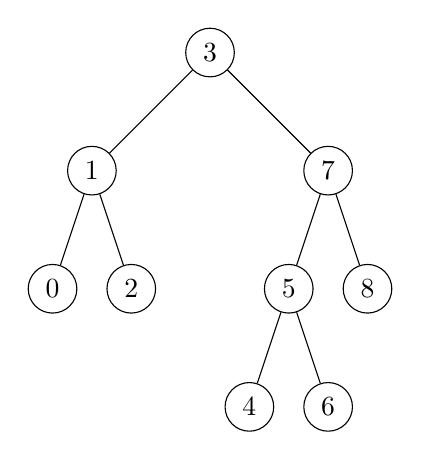
\begin{tikzpicture}
      [level 1/.style={sibling distance=30mm},
       level 2/.style={sibling distance=15mm},
       level 2/.style={sibling distance=10mm}]
      \tikzstyle{every node}=[circle,draw]
      \node{3}
      child{
        node{1}
        child{node{0}}
        child{node{2}}
      }
      child{
        node{7}
        child{
          node{5}
          child{node{4}}
          child{node{6}}
        }
        child{node{8}}
      };
    \end{tikzpicture} \hspace{4mm}
    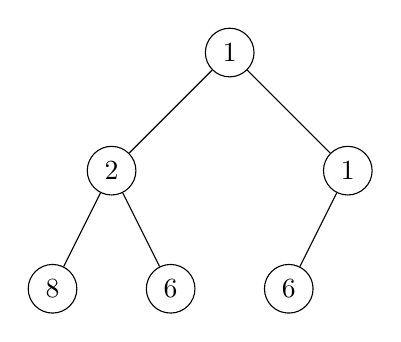
\begin{tikzpicture}
      [level 1/.style={sibling distance=30mm},
       level 2/.style={sibling distance=15mm}]
      \tikzstyle{every node}=[circle,draw]
      \node{1}
      child{
        node{2}
        child{node{8}}
        child{node{6}}
      }
      child{
        node{1}
        child{node{6}}
        child[missing]{node{k}}
      }
      ;
    \end{tikzpicture} \hspace{4mm}
    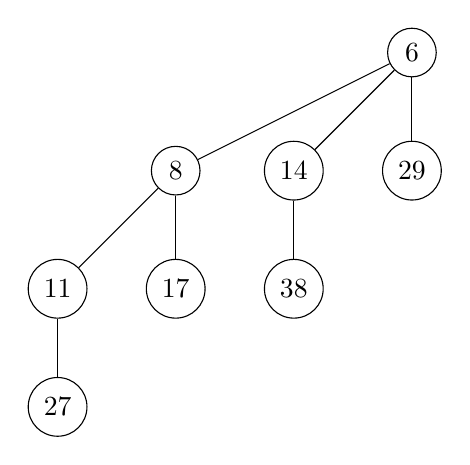
\begin{tikzpicture}[grow via three points={%
        one child at (0,-1.5) and two children at (0,-1.5) and (-1.5,-1.5)}]
      \tikzstyle{every node}=[circle,draw]
      \node at (0,0) {6}
      child{node{29}}
      child{
        node{14}
        child{
          node{38}
        }
      }
      child{
        node{8}
        child{node{17}}
        child{
          node{11}
          child{node{27}}
        }
      }
      ;
    \end{tikzpicture}
  \end{center}
  \caption{A binary search tree (on the left), a binary min-heap (in
    the middle), and a binomial tree of rank $3$ (on the right).}
  \label{fig:trees}
\end{figure}

Algorithms can be typeset as pseudo-code as exemplified in
Algorithm~\ref{algo:demo}: study its \LaTeX\ source code.

\begin{algorithm}[t]
  \begin{algorithmic}[1]  % comment [1] away to drop the line numbers
    \STATE \Function $f(n)$
    \IF[optional comment]{$n < 0$}
      \STATE $n \IsAssigned -2 \cdot n$ \COMMENT{optional comment}
    \ELSE[$n \geq 0$]
      \STATE $n \IsAssigned  3 \cdot n$
    \ENDIF
    \WHILE[optional comment]{$n > 0$}
      \STATE $n \IsAssigned n-1$
    \ENDWHILE
    \RETURN $n$
  \end{algorithmic}
  \caption{Silly algorithm}
  \label{algo:demo}
\end{algorithm}

If you are not sure whether you will stick to your current choice of
notation or terminology, then introduce a new (possibly parametric)
command.  For example, upon
\begin{center}
  \verb|\newcommand{\Cardinality}[1]{\left\lvert#1\right\rvert}|
\end{center}
the formula \verb|$\Cardinality{S}$| typesets the cardinality of set
$S$ as $\Cardinality{S}$ with autosized vertical bars and proper
spacing, but upon changing the definition of that parametric command
to
\begin{center}
  \verb|\newcommand{\Cardinality}[1]{\# #1}|
\end{center}
and recompiling, the formula \verb|$\Cardinality{S}$| typesets the
cardinality of set $S$ as $\#S$.
%
Similarly, upon
\begin{center}
  \verb|\newcommand{\MiniZinc}{\textit{Mini\-Zinc}}|
\end{center}
the text \verb|\MiniZinc\| typesets into \textit{MiniZinc},
hyphenation being only possible in the middle, but upon changing the
definition of that non-parametric command to
\begin{center}
  \verb|\newcommand{\MiniZinc}{\textsc{Mini\-Zinc}}|
\end{center}
and recompiling, the text \verb|\MiniZinc\| typesets into
\textsc{MiniZinc}.
%
You can thus obtain an arbitrary number of changes in the document
with a \emph{constant}-time change in its source code, rather than
having to perform a \emph{linear}-time find-and-replace operation
within the source code, which is painstaking and error-prone.  The
imported file \texttt{macros.tex} has a lot of useful predefined
commands about mathematics, CP, \Gecode, modelling, \MiniZinc, and
algorithms.

Use commands on positioning (such as \verb|\hspace|, \verb|\vspace|,
and \verb|\noindent|) and appearance (such as \verb|\small| for
reducing the font size, and \verb|\textit| for italics) very
sparingly, and ideally only in (parametric) commands, as the very idea
of mark-up languages such as \LaTeX\ is to let the class designer
(usually a trained professional typesetter) decide on where things
appear and how they look.  For example, \verb|\emph| (for emphasis)
compiles (outside italicised environments, such as \texttt{theorem})
into \textit{italics} under the \texttt{article} class used for this
document, but it may compile into \textbf{boldface} under some other
class.
\begin{center}
  \textbf{If you do not (need to) worry about \emph{how} things look, \\
    then you can fully focus on \emph{what} you are trying to
    express!}
\end{center}

Note that \emph{no} absolute numbers are used in the \LaTeX\ source
code for any of the references inside this document.  For ease of
maintenance, \verb|\label| is used for giving a label to something
that is automatically numbered (such as an algorithm, equation,
figure, footnote, item, line, part, section, subsection, or table),
and \verb|\ref| is used for referring to a label.  An item in the
bibliography file is referred to by \verb|\cite| instead.  Upon
changing the text, it suffices to recompile, once or twice, and
possibly to run BibTeX again, in order to update all references
consistently.

Always write
%
\verb| Table|$\sim$\verb|\ref{tab:maths} |
%
instead of
%
\verb| Table \ref{tab:maths}|,
%
by using the non-breaking space (which is typeset as the tilde $\sim$)
instead of the normal space, because this avoids that a
cross-reference is spread across a line break, as for example in
``Table \ref{tab:maths}'', which is considered poor typesetting.

The rules of English for how many spaces to use before and after
various symbols are given in Table~\ref{tab:spacing}.  Beware that
they may be very different from the rules in your native language.

\begin{table}[t]
  \centering
  \begin{tabular}{cc|c|c}
    \toprule
    \multicolumn{2}{c}{} & \multicolumn{2}{l}{number of spaces after} \\
    \cmidrule{3-4}
    \multicolumn{2}{c}{} & 0 & 1 \\
    \midrule
    \multirow{2}{*}{number of spaces before} & 0 & / - & , : ; . ! ?
    ) ] \} ' '' \% \\
    \cmidrule{2-4}
    & 1 & ( [ \{ ` `` & -- (\emph{n}-dash) --- (\emph{m}-dash) \\
    \bottomrule
  \end{tabular}
  \caption{Spacing rules of English}
  \label{tab:spacing}
\end{table}

\vfill

\noindent
\handpoint\ Feel free to report to the head teacher any other features
that you would have liked to see discussed and exemplified in this
template document.
}

\end{document}

%%% Local Variables:
%%% mode: latex
%%% TeX-master: t
%%% End:
